\subsubsection{Middleware}
\subsubsubsection{Application - Middleware}
The communication protocol between application layer and middleware layer 
\paragraph{Fire and forget} 
It is a one-way message pattern (the service sends a message without expecting 
a response). Since the application and the middleware will reside on the same 
physical node we can assume that the communication is reliable, once a message 
is sent from the application layer it arrives to the middleware layer and 
viceversa. The asynchronous communication decouples (when possible) 
the computation of the application from the computation of the middleware 
and viceversa. The standard interfaces for communication 
implemented by application layer and middleware layer enables the use of 
heterogeneous technologies for each one. Defining a standard interface 
is fundamental to abstract from the underlying technologies (implementation).

\subsubsubsection{Middleware - Middleware}

The communication between the middleware layers implies the design of different 
services. Taking into account the distributed nature of the system we have 
studied specific solutions for each service, the ideas applied come from 
well known patterns used in distributed systems:
\begin{itemize}
  \item Lamport logical clocks: in a distributed system we are interested 
in the logical sequence of the events and not the wall clock time which is 
impossible to know perfectly and could lead to synchronization errors;
  \item Lamport timestamps algorithm\footnote{Leslie Lamport \textit{Time, 
clocks, and the ordering of events in a distributed system}, ACM 21, 
pp. 558-565, July 1978}: this algorithm contains the keystone 
of each distributed service which implies a form of synchronization 
between parties;
  \item Bully algorithm: this algorithm is used in the first part of the 
shutdown process. It works dynamically and implies the election of a master 
node. 
\end{itemize}

\subsubsubsection{System Boostrap}
As pointed out in Problem Analysis (\ref{sec:pa-distribution}), the system has
to start neatly. Hence, we need to design a protocol in order to accomplish 
this goal.

The protocol is represented in figure \ref{fig:sys-bootstrap-protocol}, where:

\begin{itemize}
  \item A circle is a logical node which is composed of two layers:
    \begin{itemize}
      \item \textbf{MW}:  middleware layer
      \item \textbf{APP}: application layer
  \end{itemize}
    Since the middleware has to be application-independent, it only assumes 
    that the application layer exposes an interface through which it is 
    possible to start the application neatly;
  \item \textbf{Named arrow}: it represents a message that is sent from a 
logical node through another one with the name as its payload;
  \item \textbf{Number}: it represents the progress of the logical system clock 
during the bootstrap process.
\end{itemize}

\begin{figure}[H]
  \centering
  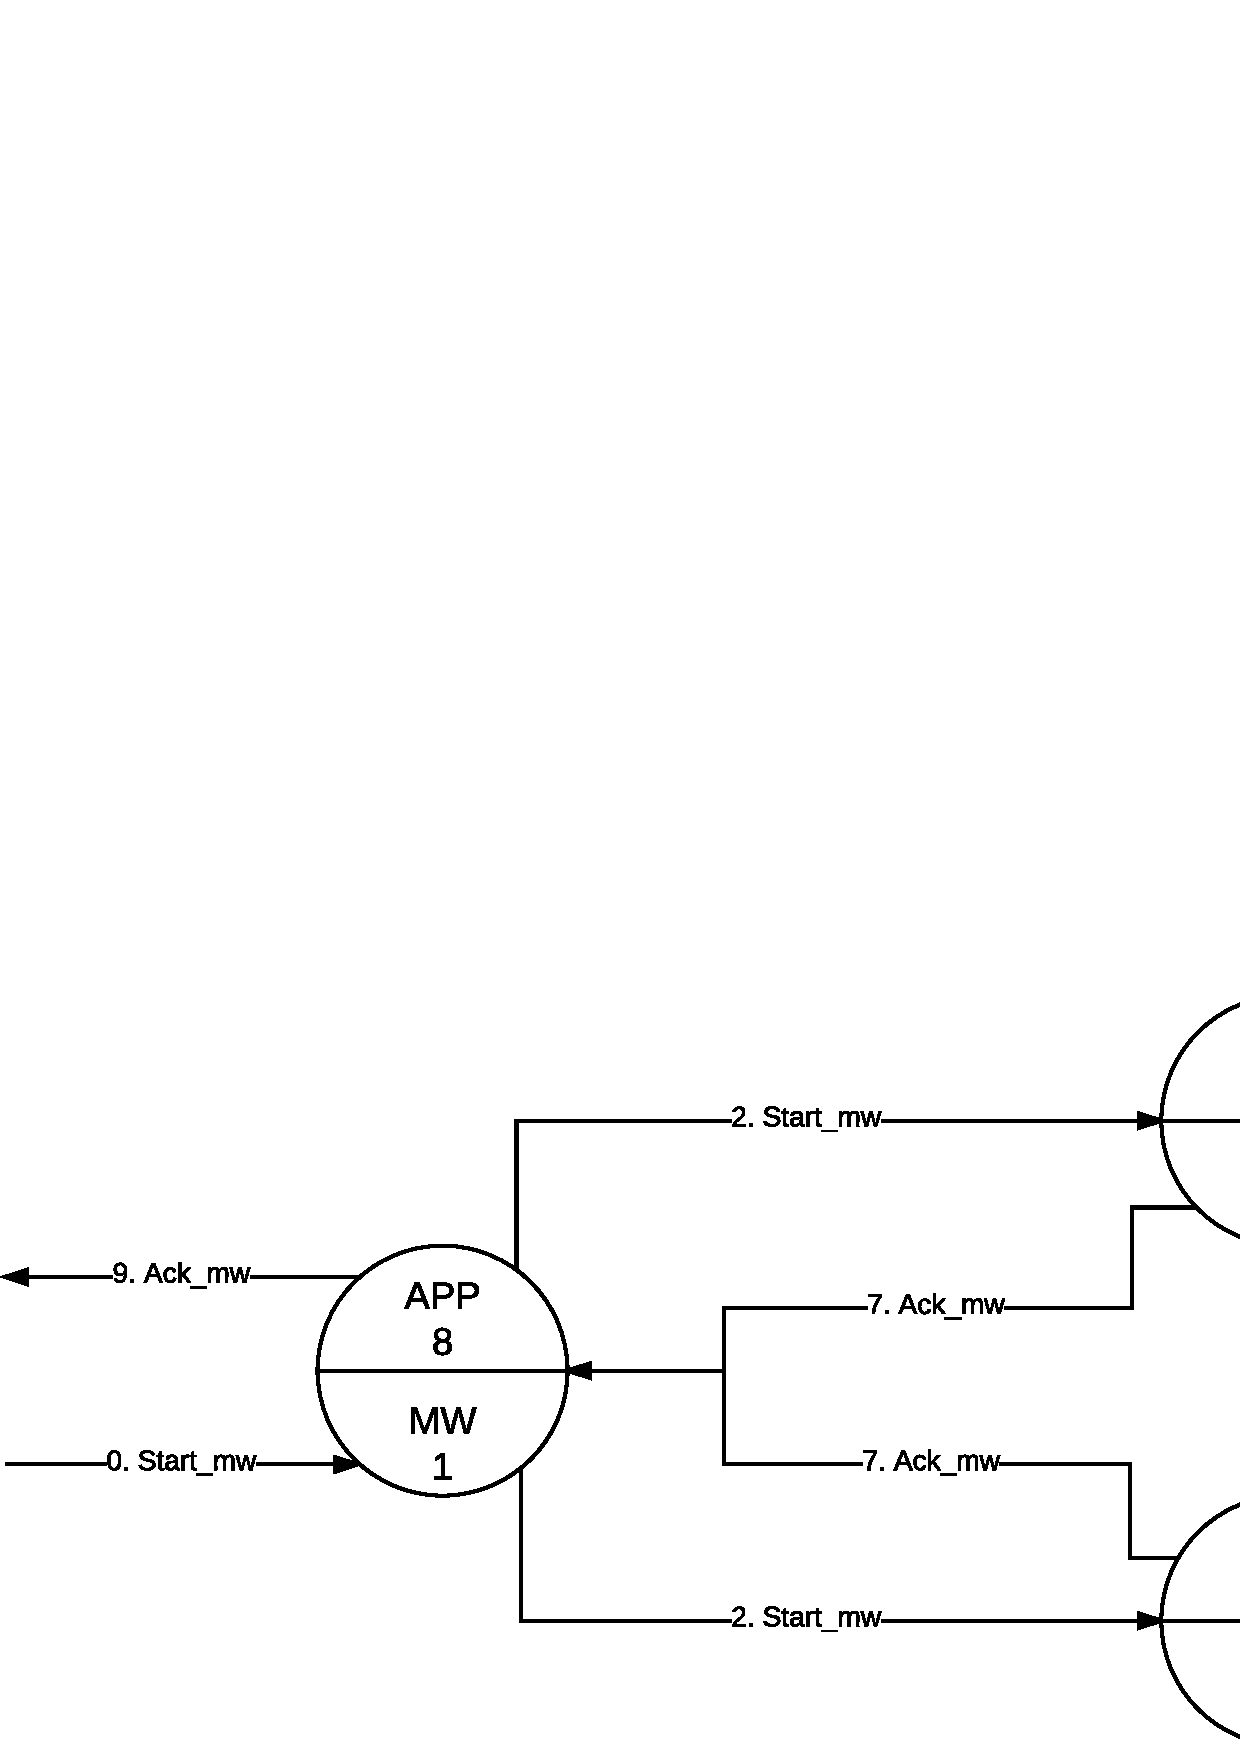
\includegraphics[width=\columnwidth]{sections/images/solution/bootstrap.pdf}
  \caption{System bootstrap protocol}
  \label{fig:sys-bootstrap-protocol}
\end{figure}

Assuming that a \texttt{Start\_mw} message arrives to a non-booted node (say
$l$) at time 0, the protocol is defined as follows:

\begin{enumerate}
  \item The leftmost node $l$ in figure \ref{fig:sys-bootstrap-protocol}
    starts its own middleware services.  
  \item $l$ sends a \texttt{Start\_mw} message to the set $S$ of all its
    neighbors. Clearly, if it was the first node in the system to receive
    \texttt{Start\_mw}, then it will be also the last node to complete the
    boot process.
  \item $l$ waits for each node in $S$ to complete the boot. $l$ waits for all
nodes in $S$ to send an \texttt{Ack\_mw} message back;
  \item The middleware MW of $l$ grants the application APP to start;
  \item $l$ then sends an \texttt{Ack\_mw} message back.
\end{enumerate}

As it can be seen in the figure, this behaviour is replicated recursively
by all nodes of the system. If a node has already been booted, then it only
sends \texttt{Ack\_mw} back.

\subsubsubsection{System Termination}
Also, the system has to shutdown neatly. Therefore we designed a protocol to
stop the entire system; please notice that this one could be seen as a
symmetric version of the System Bootstrap protocol.
% TODO: please check the sentence here above

The protocol is represented in figure \ref{fig:sys-termination-protocol}, where
the conventions are the same as the ones used in figure
\ref{fig:sys-bootstrap-protocol}.

\begin{figure}[H]
  \centering
  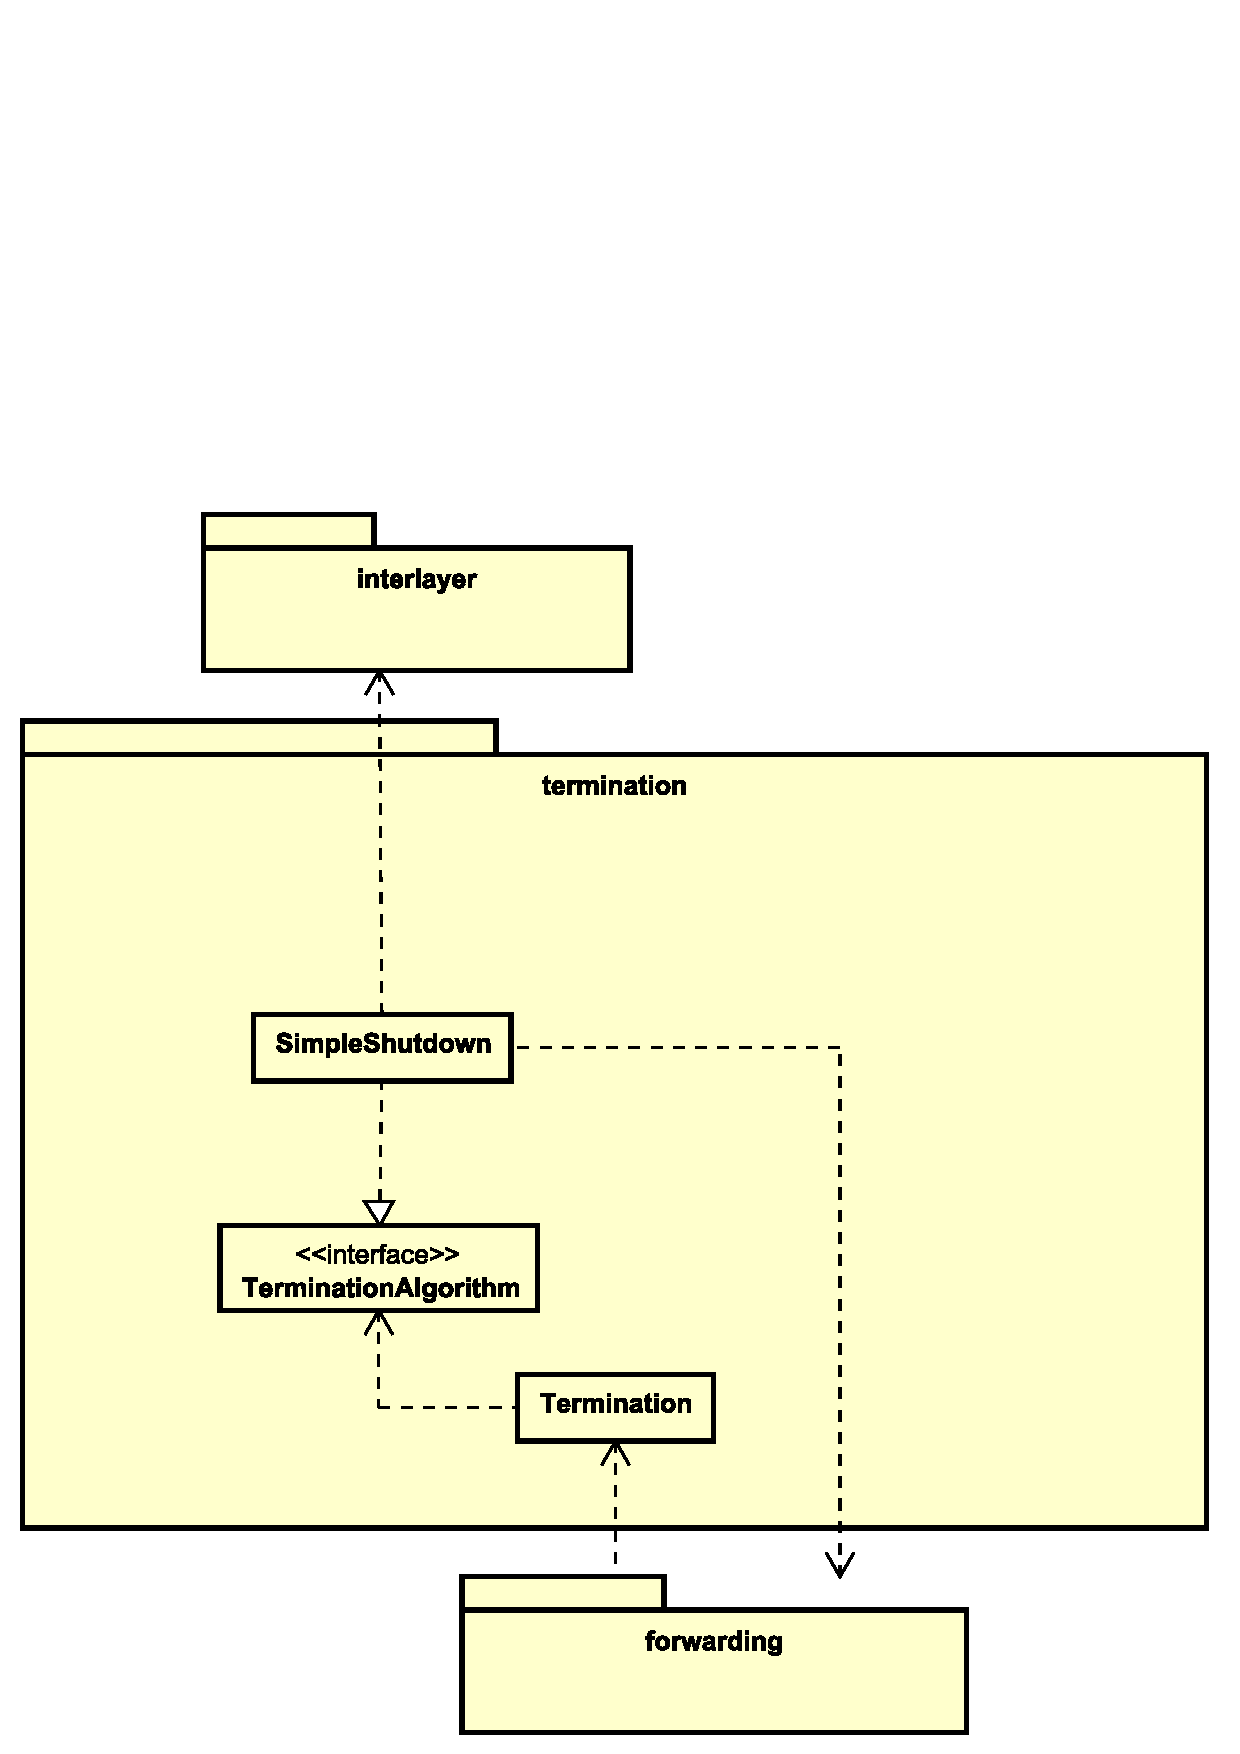
\includegraphics[width=\columnwidth]{sections/images/solution/termination.pdf}
  \caption{System termination protocol}
  \label{fig:sys-termination-protocol}
\end{figure}

Assuming that a \texttt{Shutdown\_mw} message arrives to a non-terminated node
$l$ (let it be the leftmost one in the picture) at time instant 0, the protocol
is defined as follows:

\begin{enumerate}
  \item The middleware MW of $l$ asks to terminate the application APP;
  \item $l$ sends a \texttt{Shutdown\_mw} message to the set
    $S$ of all the nodes it knows;
  \item $l$ waits for each node in $S$ to terminate, i.e. $l$ waits for all
    nodes in $S$ to send an \texttt{Ack\_mw} message back;
  \item $l$ stops its own middleware services;
  \item $l$ then sends an \texttt{Ack\_mw} message back.
\end{enumerate}

As it can be seen in the related figure, this behaviour is replicated
recursively by all nodes of the system. If a node has already terminated, then
it only sends \texttt{Ack\_mw} back.
